\documentclass[border=10pt]{standalone}
\usepackage{tikz}
\usetikzlibrary{arrows.meta, positioning, calc, fit, backgrounds}
\usepackage{xcolor}
\usepackage{helvet}
\renewcommand{\familydefault}{\sfdefault}

\definecolor{inputcol}{HTML}{E8EAF6}
\definecolor{cnncol}{HTML}{C5CAE9}
\definecolor{cnnborder}{HTML}{5C6BC0}
\definecolor{tokencol}{HTML}{FFF3E0}
\definecolor{tokenborder}{HTML}{FB8C00}
\definecolor{attncol}{HTML}{E8F5E9}
\definecolor{attnborder}{HTML}{43A047}
\definecolor{headcol}{HTML}{FCE4EC}
\definecolor{headborder}{HTML}{E91E63}
\definecolor{flatcnncol}{HTML}{BBDEFB}
\definecolor{flatcnnborder}{HTML}{1E88E5}
\definecolor{poolcol}{HTML}{F3E5F5}
\definecolor{poolborder}{HTML}{8E24AA}
\definecolor{labelcol}{HTML}{37474F}
\definecolor{dimcol}{HTML}{78909C}
\definecolor{auxcol}{HTML}{D1C4E9}
\definecolor{auxborder}{HTML}{7E57C2}

\begin{document}
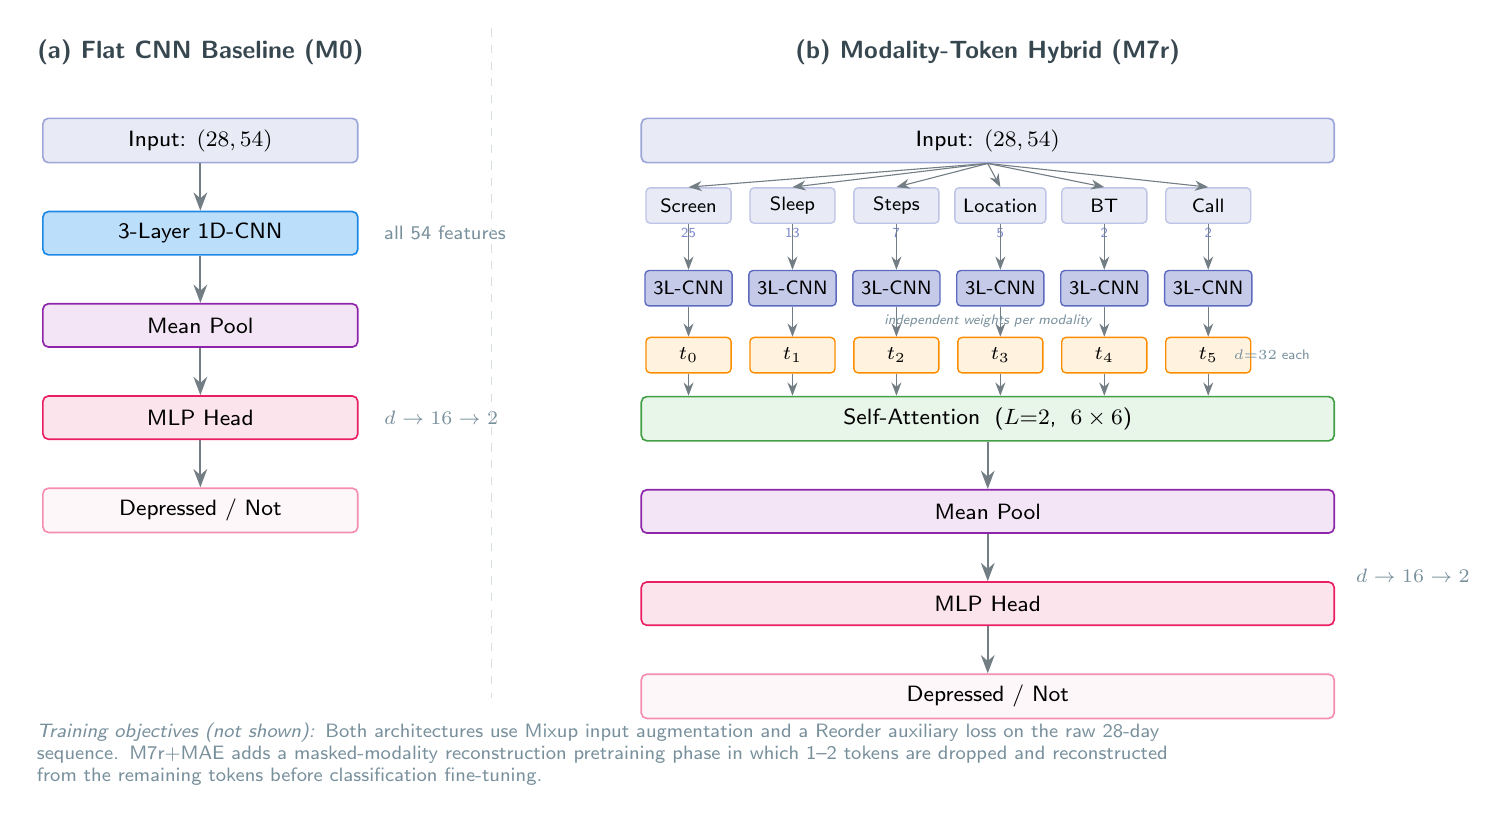
\begin{tikzpicture}[
    >=Stealth,
    box/.style={draw, rounded corners=2pt, minimum height=0.55cm, inner sep=4pt, 
        font=\footnotesize\sffamily, align=center, line width=0.6pt},
    smallbox/.style={draw, rounded corners=1.5pt, minimum height=0.45cm, inner sep=3pt, 
        font=\scriptsize\sffamily, align=center, line width=0.5pt},
    ann/.style={font=\scriptsize\sffamily, text=dimcol},
    heading/.style={font=\small\bfseries\sffamily, text=labelcol},
    arrow/.style={->, thick, color=labelcol!70},
]

% ============================================================
%  (a) Flat CNN Baseline (M0)
% ============================================================
\node[heading] (titleA) at (0, 0) {(a) Flat CNN Baseline (M0)};

\node[box, fill=inputcol, draw=cnnborder!60, minimum width=4cm, below=0.55cm of titleA] 
    (inA) {Input: $(28, 54)$};

\node[box, fill=flatcnncol, draw=flatcnnborder, minimum width=4cm, below=0.6cm of inA] 
    (cnnA) {3-Layer 1D-CNN};
\node[ann, right=0.2cm of cnnA] {all 54 features};

\node[box, fill=poolcol, draw=poolborder, minimum width=4cm, below=0.6cm of cnnA] 
    (poolA) {Mean Pool};

\node[box, fill=headcol, draw=headborder, minimum width=4cm, below=0.6cm of poolA] 
    (mlpA) {MLP Head};
\node[ann, right=0.2cm of mlpA] {$d \to 16 \to 2$};

\node[box, fill=headcol!30, draw=headborder!50, minimum width=4cm, below=0.6cm of mlpA] 
    (outA) {Depressed / Not};

\draw[arrow] (inA) -- (cnnA);
\draw[arrow] (cnnA) -- (poolA);
\draw[arrow] (poolA) -- (mlpA);
\draw[arrow] (mlpA) -- (outA);


% ============================================================
%  (b) Modality-Token Hybrid (M7r)
% ============================================================
\node[heading] (titleB) at (10, 0) {(b) Modality-Token Hybrid (M7r)};

\node[box, fill=inputcol, draw=cnnborder!60, minimum width=8.8cm, below=0.55cm of titleB] 
    (inB) {Input: $(28, 54)$};

% --- Modality split row ---
\def\mods{{"Screen","Sleep","Steps","Location","BT","Call"}}
\def\dims{{"25","13","7","5","2","2"}}
\def\xstart{6.2}
\def\xstep{1.32}

\foreach \i in {0,...,5} {
    \pgfmathsetmacro{\xp}{\xstart + \i*\xstep}
    \pgfmathsetmacro{\mn}{\mods[\i]}
    \pgfmathsetmacro{\dv}{\dims[\i]}

    \node[smallbox, fill=inputcol, draw=cnnborder!40, minimum width=1.08cm] 
        (sl\i) at (\xp, -1.95) {\scriptsize \mn};
    \node[font=\tiny\sffamily, text=cnnborder!80] at (\xp, -2.3) {\dv};
}

% Fan-out arrows from input
\foreach \i in {0,...,5} { \draw[arrow, thin] (inB.south) -- (sl\i.north); }

% --- CNN encoder row ---
\foreach \i in {0,...,5} {
    \pgfmathsetmacro{\xp}{\xstart + \i*\xstep}
    \node[smallbox, fill=cnncol, draw=cnnborder, minimum width=1.08cm] 
        (enc\i) at (\xp, -3.0) {\scriptsize 3L-CNN};
    \draw[arrow, thin] (sl\i) -- (enc\i);
}

% --- Token row ---
\foreach \i in {0,...,5} {
    \pgfmathsetmacro{\xp}{\xstart + \i*\xstep}
    \node[smallbox, fill=tokencol, draw=tokenborder, minimum width=1.08cm] 
        (tk\i) at (\xp, -3.85) {\scriptsize $t_{\pgfmathprintnumber{\i}}$};
    \draw[arrow, thin] (enc\i) -- (tk\i);
}

% Single concise annotation for the encoder block
% Annotations centered below rows
\node[ann, font=\tiny\itshape] at (10, -3.42) {independent weights per modality};
\node[ann, font=\tiny, anchor=west] at (13.0, -3.85) {$d{=}32$ each};

% --- Self-attention ---
\node[box, fill=attncol, draw=attnborder, minimum width=8.8cm, below=2.95cm of inB] 
    (attn) {Self-Attention \;($L{=}2$,\; $6 \times 6$)};

\foreach \i in {0,...,5} { \draw[arrow, thin] (tk\i) -- (attn.north -| tk\i); }

% --- Mean Pool ---
\node[box, fill=poolcol, draw=poolborder, minimum width=8.8cm, below=0.6cm of attn] 
    (poolB) {Mean Pool};

% --- MLP Head ---
\node[box, fill=headcol, draw=headborder, minimum width=8.8cm, below=0.6cm of poolB] 
    (mlpB) {MLP Head};
\node[ann, anchor=west] at (14.55, -6.65) {$d \to 16 \to 2$};

% --- Output ---
\node[box, fill=headcol!30, draw=headborder!50, minimum width=8.8cm, below=0.6cm of mlpB] 
    (outB) {Depressed / Not};

\draw[arrow] (attn) -- (poolB);
\draw[arrow] (poolB) -- (mlpB);
\draw[arrow] (mlpB) -- (outB);

% ============================================================
%  Divider
% ============================================================
\draw[dashed, color=dimcol!30, line width=0.5pt] (3.7, 0.3) -- (3.7, -8.2);

% ============================================================
%  Training note (below both panels)
% ============================================================
\node[anchor=north west, text width=14.5cm, font=\scriptsize\sffamily, text=dimcol] 
    at (-2.2, -8.4) {%
    \textit{Training objectives (not shown):}
    Both architectures use Mixup input augmentation and a Reorder auxiliary loss on the raw 28-day sequence.
    M7r+MAE adds a masked-modality reconstruction pretraining phase in which 1--2 tokens are dropped 
    and reconstructed from the remaining tokens before classification fine-tuning.%
    };

\end{tikzpicture}
\end{document}
